\section{Opérateurs de traitement d'images}
À l’instar des opérateurs mathématiques, les opérateurs de traitement d’images prennent en entrée une image et un ensemble d’informations relatives à cette image, effectuent des modifications sur ces entrées et retournent une nouvelle image ou un ensemble d’informations relatives aux données d’entrée. Ces opérateurs sont nombreux. Mais nous allons en citer quelques-uns.
    \subsection{Opérateurs morpho-mathématiques}
Les opérateurs morpho-mathématiques sont des opérations qui traitent des images en fonction de formes. Elles appliquent un élément structurant à une image d'entrée, créant une image de sortie de même taille. Dans une opérateur morphologique, la valeur de chaque pixel de l'image de sortie est basée sur une comparaison du pixel correspondant de l'image d'entrée avec ses voisins. Elles peuvent être utilisées pour supprimer les bruits sur une image. Les principales opérateurs morphologiques sont:
    \begin{itemize}
        \item[•]\textbf{La dilatation}: la valeur du pixel de sortie est la valeur maximale de tous les pixels du voisinage. Dans une image binaire, un pixel est défini sur 1 si l'un des pixels voisins a la valeur 1. La dilatation morphologique rend les objets plus visibles et comble les petits trous dans les objets.
        \begin{figure}[H]
            \centering
            
\includegraphics[scale=0.7]{dilatation}
            \caption{Dilatation}
        \end{figure}  
       
        \item[•]\textbf{L'érosion}: la valeur du pixel de sortie est la valeur minimale de tous les pixels du voisinage. Dans une image binaire, un pixel est défini sur 0 si l'un des pixels voisins a la valeur 0. L'érosion morphologique supprime les îles et les petits objets de sorte que seuls les objets substantifs restent. 
        \begin{figure}[H]
            \centering
            
\includegraphics[scale=0.7]{erosion}
            \caption{Érosion}
        \end{figure}  
        \item[•]\textbf{L'ouverture}: l'opération d'ouverture érode une image puis dilate l'image érodée, en utilisant le même élément structurant pour les deux opérations. L'ouverture morphologique est utile pour supprimer les petits objets d'une image tout en préservant la forme et la taille des objets plus gros dans l'image. 
            \begin{figure}[H]
                \centering
                
\includegraphics[scale=0.5]{opening}
                \caption{Ouverture}
            \end{figure} 
        \item[•]\textbf{La fermeture}: l'opération de fermeture dilate une image puis érode l'image dilatée, en utilisant le même élément structurant pour les deux opérations. La fermeture morphologique est utile pour combler les petits trous d'une image tout en préservant la forme et la taille des objets de l'image.\cite{mathlabMorpho}
        \begin{figure}[H]
            \centering
            
\includegraphics[scale=0.5]{closing}
            \caption{Fermeture}
        \end{figure} 
    \end{itemize} 

    \subsection{Détection des contours}
    La détection de contours est une étape essentielle du processus de traitement d’images qui permet une réduction importante de la quantité d’information relative à une image, tout en préservant des informations structurelles comme les contours et les frontières des images. Elle consiste à repérer les points d'une image numérique qui correspondent à un
    changement brutal de l'intensité lumineuse. En effet, un contour se matérialise par une rupture d'intensité
    dans l'image suivant une direction donnée. Plusieurs méthodes existent pour détecter cette rupture, les unes plus ou moins complexes, les autres plus ou moins gourmandes en calcul.

    \begin{itemize}
        \item[•]\textbf{Le filtre de Prewitt}: Prewitt est l'un des premiers algorithmes de détection de contours dans le domaine du traitement d'image.
        Il s'agit d'une approximation du gradient par convolution de l'image avec des masques de convolution.
        \item[•]\textbf{Le filtre de Sobel} : le filtre de Sobel détecte séparément les bords horizontaux et verticaux sur une image en niveaux de gris. Et on peut aussi appliquer le détecteur de Sobel sur des images en couleurs en appliquant le même
        algorithme sur les différentes composantes RGB prises séparément.
        \item[•]\textbf{Le filtre de Canny} : la méthode de Canny implémente une estimation du gradient de l'image à l'aide du filtre de Sobel, suivi
        d'un seuillage par hystérésis du module de gradient. Un seuil haut et un seuil bas sont à définir.
        Tous les pixels où le module du gradient est supérieur au premier seuil sont classifiés comme appartenant
        aux contours de l'image, des contours de l'image sont ainsi formés. Les pixels ayant un module supérieur
        au seuil bas et qui sont segmentés précédents sont définis comme points de contour dans l'image binaire
        résultante.\cite{akacemMaster}
    \end{itemize}
    \begin{figure}[H]
        \begin{subfigure}{0.3\textwidth}
            \centering
            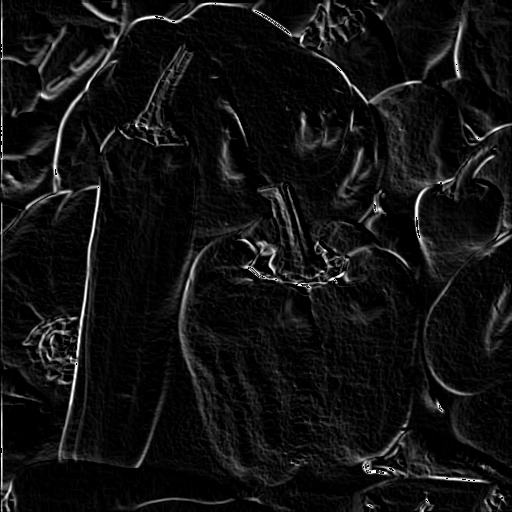
\includegraphics[width=\textwidth]{food_prewitt}
            \caption{Filtre de Prewitt}
        \end{subfigure}
        \hfill
        \begin{subfigure}{0.3\textwidth}
            \centering
            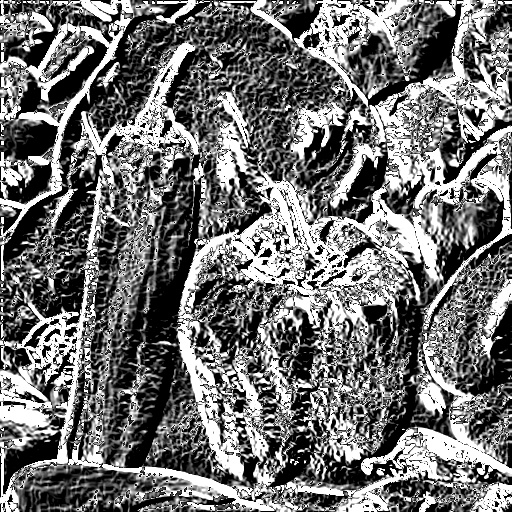
\includegraphics[width=\textwidth]{food_sobel}
            \caption{Filtre de Sobel}
        \end{subfigure}
        \hfill
        \begin{subfigure}{0.3\textwidth}
            \centering
            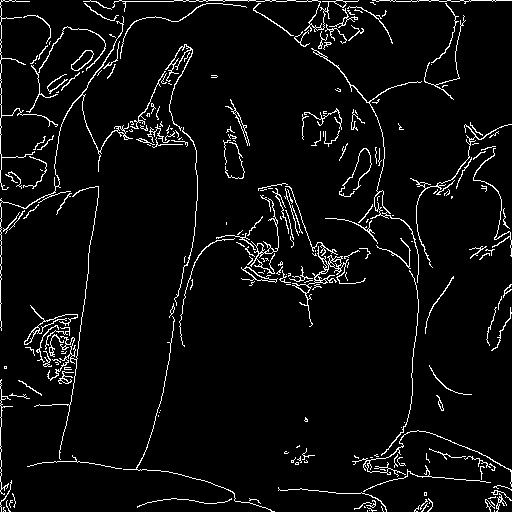
\includegraphics[width=\textwidth]{food_canny}
            \caption{Filtre de Canny}
        \end{subfigure}
        \caption{Détection des contours avec différents filtres}
    \end{figure}

